% You should title the file with a .tex extension (hw1.tex, for example)
\documentclass[11pt]{article}

\usepackage{hyperref}
\usepackage{amsmath}
\usepackage{mathtools}
\usepackage{amssymb}
\usepackage{wrapfig}
\usepackage{fancyhdr}
\usepackage{tikz-qtree}
\usepackage{tikz-qtree-compat}
\usepackage[normalem]{ulem}
\usepackage{tikz}
\usepackage{graphicx}
\DeclareMathOperator*{\argmin}{argmin}
\DeclareMathOperator*{\argmax}{argmax}

\oddsidemargin0cm
\topmargin-2cm     %I recommend adding these three lines to increase the 
\textwidth16.5cm   %amount of usable space on the page (and save trees)
\textheight23.5cm  

\newcommand{\question}[2] {\vspace{.25in} \hrule\vspace{0.5em}
\noindent{\bf #1: #2} \vspace{0.5em}
\hrule \vspace{.10in}}
\renewcommand{\part}[1] {\vspace{.10in} {\bf (#1)}}

\newcommand{\myname}{Sean Bittner}
\newcommand{\myandrew}{srb2201@columbia.edu}
\newcommand{\myhwnum}{12}

\setlength{\parindent}{0pt}
\setlength{\parskip}{5pt plus 1pt}
 
\DeclarePairedDelimiter\abs{\lvert}{\rvert}%
 %
\pagestyle{fancyplain}
\rhead{\fancyplain{}{\myname\\ \myandrew}}

\begin{document}

\medskip                        % Skip a "medium" amount of space
                                % (latex determines what medium is)
                                % Also try: \bigskip, \littleskip

\thispagestyle{plain}
\begin{center}                  % Center the following lines
{\Large Degenerate parametric distributions of a model of superior colliculus performing flexible routing} \\
Sean Bittner \\
March 8, 2019 \\
\end{center}

\section{Introduction}
\noindent Our collaborators (Duan et al. 2019, in prep.), have compelling data suggesting that superior colliculus (SC) is involved in flexible routing of information.  They have designed a nonlinear dynamical model of SC, and seek to characterize the parameterizations that reproduce the emergent properties of their dataset.  They have already performed a simulate-then-characterize based analysis that has provided substantial insight.  We will explore how degenerate solution networks (DSNs) can provide deeper insight about the model through the full distribution of model parameterizations, which reproduces the experimental findings.

In the manuscript, satisfactory model parameterizations are found from many initializations.  Statements about the sign of connectivity parameters (the excitatory or inhibitory nature of these projections) are made based on counts from the 373 total parameterizations (e.g. PRO $\leftrightarrow$ ANTI same hemisphere are almost always inhibitory, or PRO $\leftrightarrow$ ANTI cross hemisphere are almost always excitatory).  The goal here with DSNs is to use machine learning to learn a proabilitistic mapping from parameter space to task performance (and other properties) in a way that is optimized to find all possible parameterizations.  Once a DSN is optimized, we can effectively sample arbitarily many times from this degenerate parameteric distribution.  This allows greater statistical power for statements on the probability of weight sign, shur mode contribution, or even implications on behavior in less-probable regions of parameter space (e.g. excitatory PRO $\leftrightarrow$ ANTI same hemisphere connections).  Since DSNs are optimized to identify the full (maximum entropy) distribution of parameterizations, they may reveal new, unexpected solutions, whose mechanistic implementation of the flexible routing computation may be scientifically relevant.

\section{Method: Degenerate solution networks (DSNs)}
Theoretical neuroscientists seek to design models or find parameterizations of models that yield emergent properties of behavior.  These emergent properties (or high-level descriptions) of behavior contrast with say a collection of raw data points from an experiment.  We have a host of methods from Bayesian machine learning that learn posteriors conditioning on a collection of experimentally collected data points. But, how do we do inference conditioned on statistically defined emergent properties of interest?  We have developed a novel machine learning methodology for training degenerate solution networks (DSNs), which learn the full (i.e. maximum entropy) distribution of model parameterizations that yield a statistically defined behavior of interest.  DSNs are trained to emit samples of maximum entropy distributions of model parameters, along with the density of such samples, and are thusly termed ``density" networks.  DSNs were designed to be a tool for theoretical neuroscientists enabling exploratory analyses, and scientific hypothesis testing with models.
 
Consider model parameterization $z$ and data $x$ generated from the model $p(x \mid z)$  with known sampling procedure.  To train a DSN, the actual likelihood of this model may or may not be known.  For example, in the nonlinear dynamical SC model, there is a known sampling procedure for simulating activity given the circuit parameterization, yet an explicit likelihood function for the generated 
\begin{wrapfigure}{l}{.45\textwidth}
 \caption{\label{fig:fig1} Degenerate solution network}
  \begin{center}  
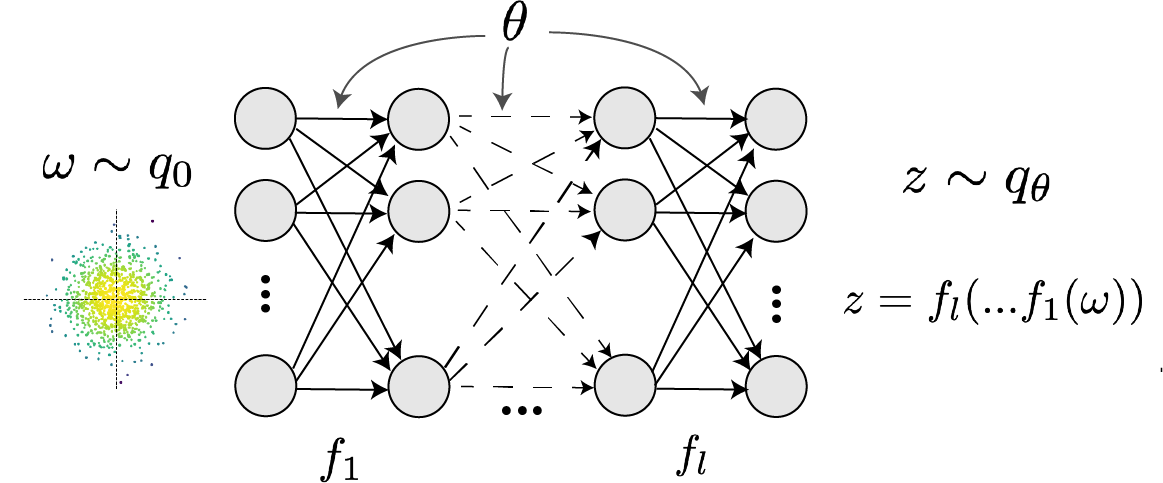
\includegraphics[scale=.3]{figs/DSN.png} 
\end{center}
 \end{wrapfigure}
 neural activity is unavailable due to the complex nonlinear dynamics.  In deep generative density networks, a simple random variable $w \sim p_0$ is mapped deterministically via a function $f_\theta$ parameterized by a neural network to the support of the distribution of interest where $z = f_{\theta}(w)$.  Given a model $p(x \mid z)$ and some behavior of interest $\mathcal{B}: E_{z \sim q_\theta}\left[ E_{x\sim p(x \mid z)}\left[T(x)\right] \right] = \mu$, DSNs are trained by optimizing the deep generative parameters $\theta$ to find the optimal approximation $q_{\theta}^*$ within the deep generative variational family $Q$ to $p(z \mid \mathcal{B})$. This procedure is loosely equivalent to variational inference (VI) using a deep generative variational family with respect to the likelihood of the mean sufficient statistics rather than the data itself \cite{loaiza2017maximum, bittner2019learning}.  In most settings (especially those relevant to theoretical neuroscience) the likelihood of the behavior with respect to the model parameters $p(T(x) \mid z)$ is unknown or intractable, requiring an alternative to stochastic gradient variational bayes \cite{kingma2013auto} or black box variational inference \cite{ranganath2014black}. Instead, DSNs are optimized with the following objective for a given model and statistical constraints on its produced activity:
\begin{equation}
\begin{split}
q_\theta^*(z) &= \argmax_{q_\theta \in Q} H(q_\theta(z)) \\
 &  \text{s.t.  } E_{z \sim q_\theta}\left[ E_{x\sim p(x \mid z)}\left[T(x)\right] \right] = \mu \\
 \end{split}
\end{equation}
For the SC model, the means and variances of steady state responses across conditions would be reflected as first and second moment constraints on those sufficient statistics in $\mathcal{B}$.  We use an augmented Lagrangian \cite{bertsekas2014constrained} constrained optimization procedure to train the DSN.

\subsection{Example: 2-D linear system}
\begin{wrapfigure}{h}{.5\textwidth}
\vspace{-.8cm}
 \caption{\label{fig:fig2} Pairplot of oscillating 2D linear system degenerate parameterization distribution.}
  \begin{center}  
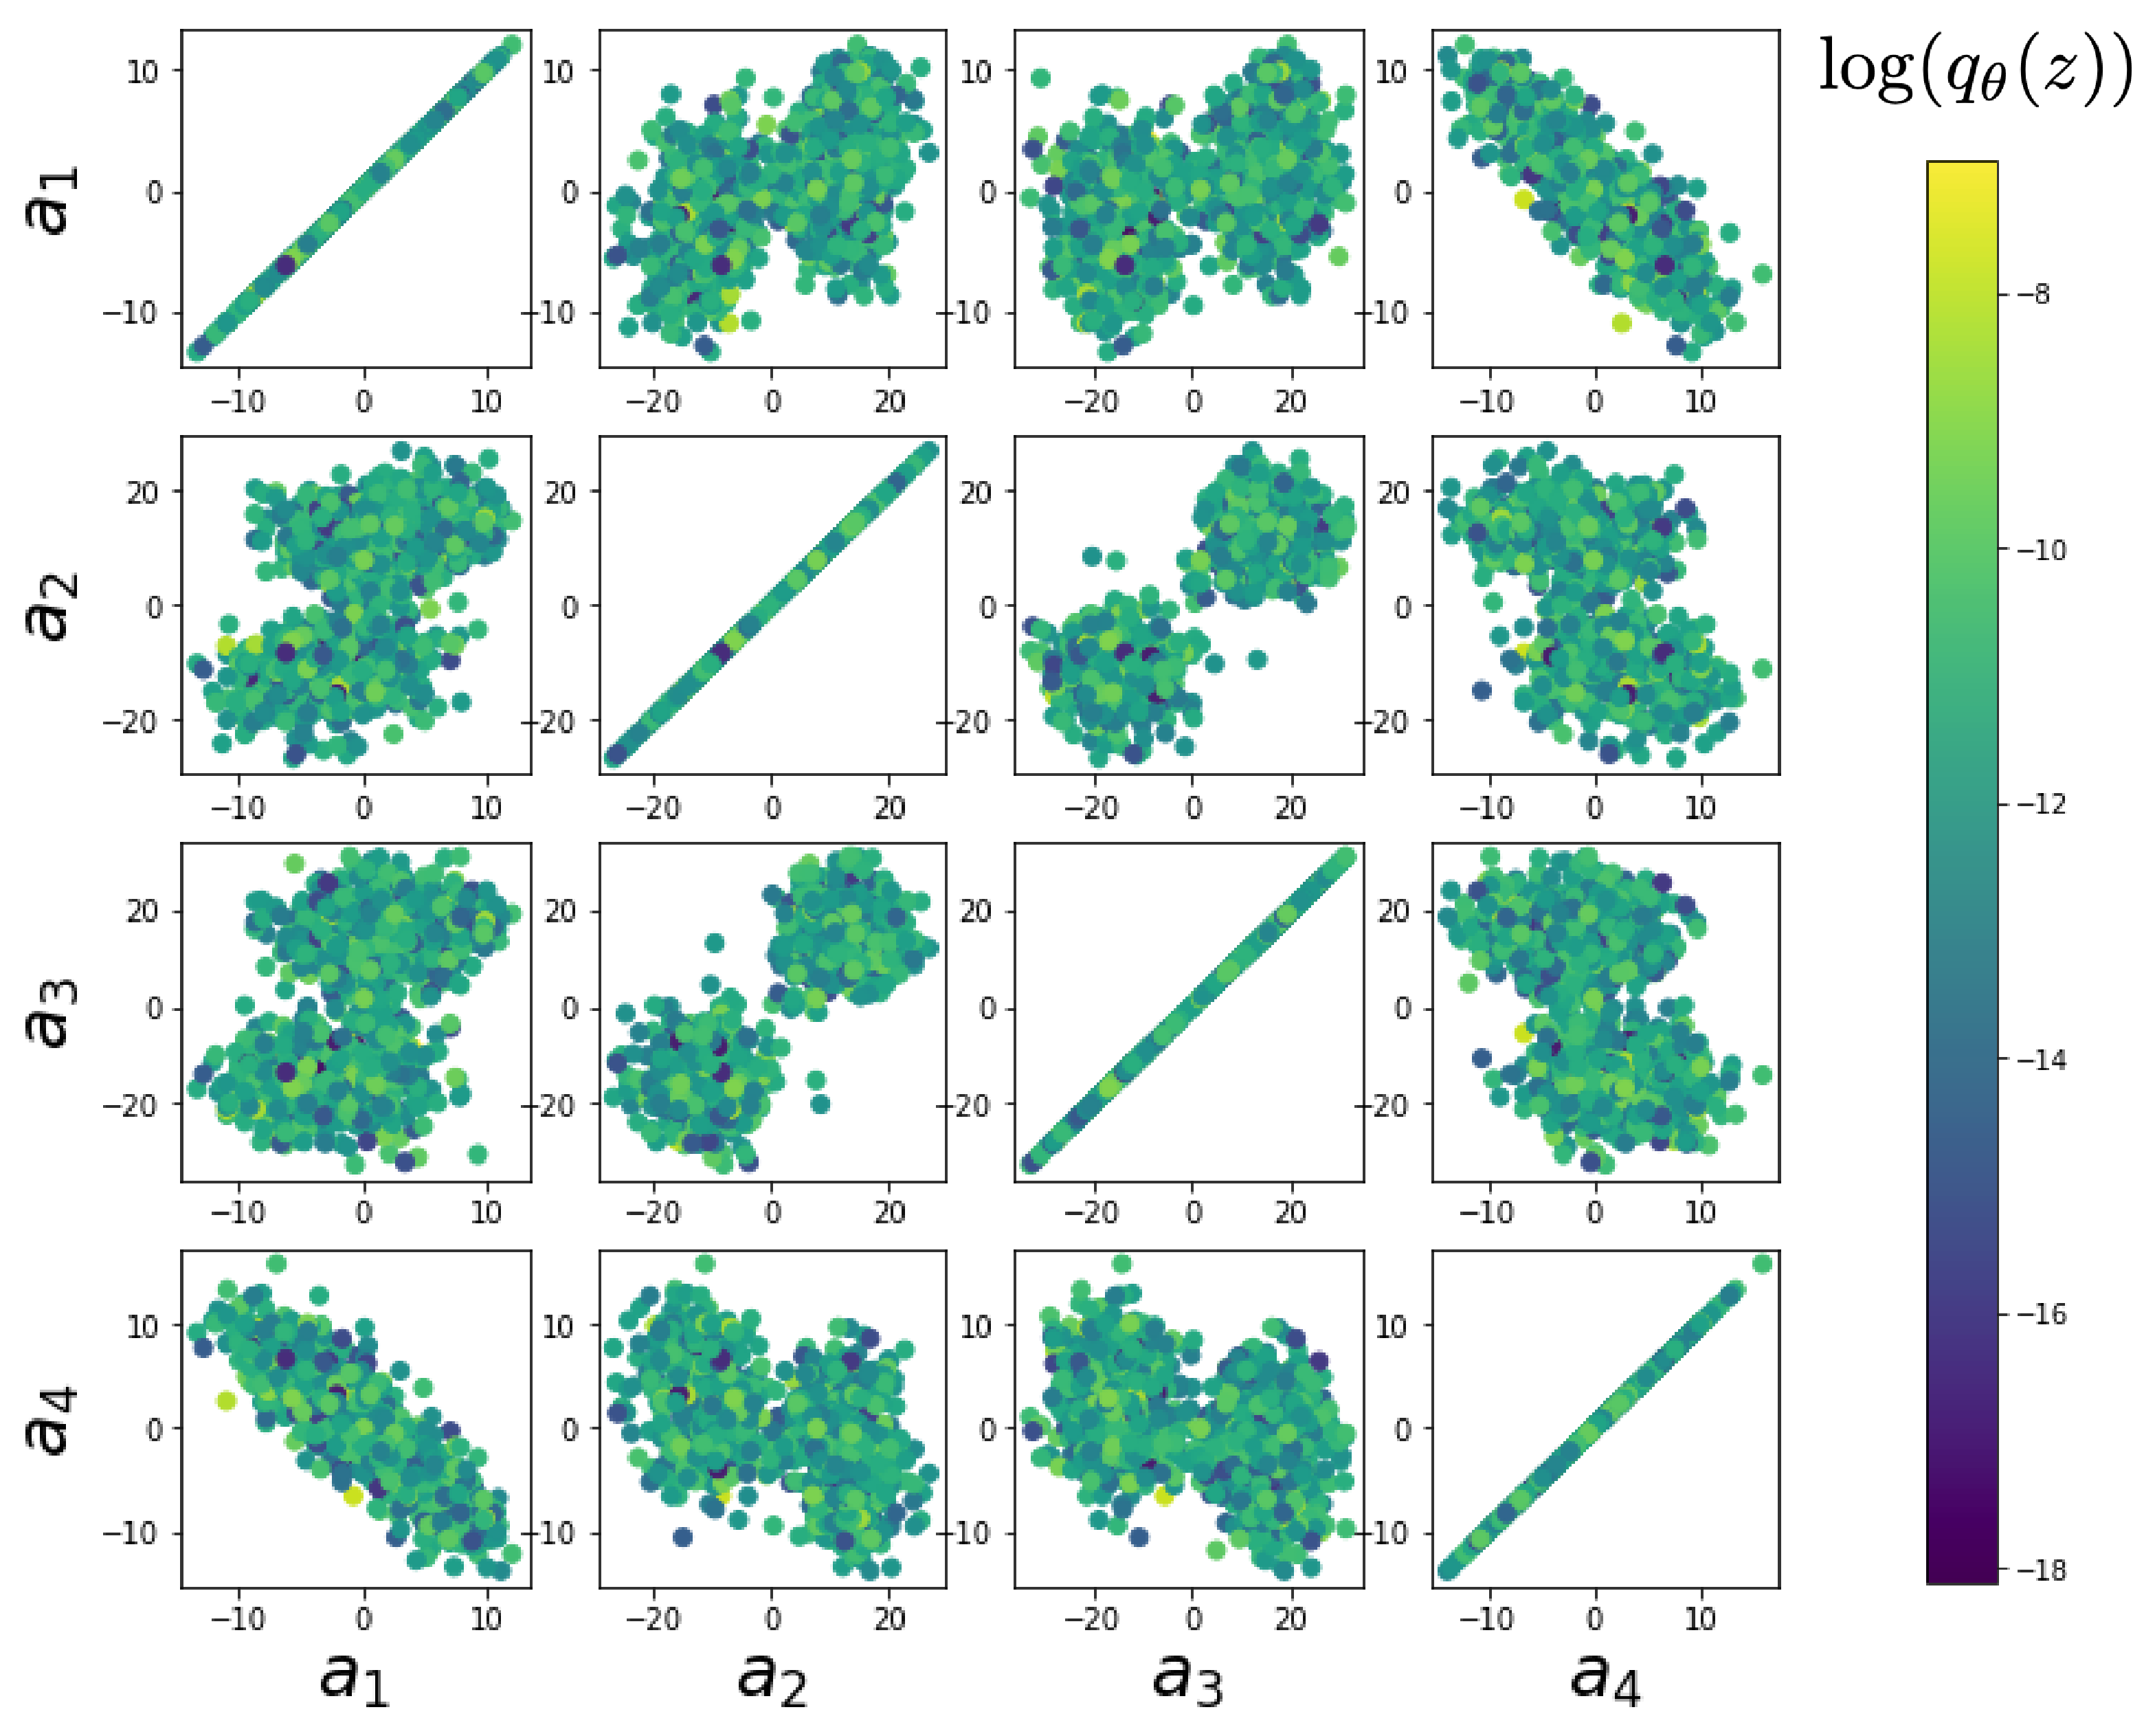
\includegraphics[scale=.3]{figs/Fig2.png} 
\end{center}
\vspace{-2cm}
\end{wrapfigure}
To gain intuition for DSNs, consider degenerate parameterizations of two-dimensional linear dynamical systems, $\tau \dot{x} = Ax$ with $A = \begin{bmatrix} a_1 & a_2 \\ a_3 & a_4 \end{bmatrix}$ that produce a band of oscillations. To train a DSN to learn the maximally entropic distribution of real entries of the dynamics matrix $z = \left[a_1, a_2, a_3, a_4 \right]$ that yield a band of oscillations, $T(x)$ is chosen to contain the first- and second-moments of the oscillatory frequency $\omega$ and the the primary growth/decay factor $c$ of the oscillating system.  To learn the distribution of real entries of A that yield a $c$ around zero with variance 1.0, and oscillations at 1 Hz with variance 0.025, the behavior of DSN is constrained to:
\begin{equation}
 \mu = E \begin{bmatrix} c \\ \omega \\ c^2 \\ \omega^2 \end{bmatrix} = \begin{bmatrix} 0.0 \\ 1.0 \\ 1.0 \\ 1.025 \end{bmatrix}
 \end{equation} 

We trained a DSN to learn the degenerate linear system parameterization (Fig. 2). Even this relatively simple system has nontrivial (though intuitively sensible) structure in the parameter distribution.  Indeed, more subtle model-behavior combinations will have even more complexity, further motivating DSNs. \\

\section{Experimental motivation}
This section briefly summarizes my understanding of the experimental motivation of SC model.  If I have misunderstood anything, or missed something important, please let us know!

Task: Cue indicates Pro or Anti condition.  Following a delay after the cue, the mouse is supposed to lick right/left if the light stimulus is on the right/left in the Pro condition, and left/right in the Anti condition.  

Electrophysiological recordings from SC and PFC indicate a much stronger encoding of task context in SC than PFC, and a significantly earlier representation of choice than PFC.  This is discordant with the prevailing understanding that PFC sends the output of flexible routing to SC.

SC neurons can be succinctly sorted into two groups -- cue neurons and delay/choice neurons by the period (before and after cue removal, respectively) of the task in which they strongly encode task context.  Furthermore, these delay/choice neurons have relatively distorted representations of task context on error trials.

There was a surprisingly high fidelity match between Pro-tuned neurons and Contra-response-tuned neurons, and between Anti-tuned neurons and Ipsi-response-tuned neurons.

During bilateral SC silencing experiments, performance was unnaffected during task cue and choice period silencing.  In delay period inactivation experiments, only performance in the Anti condition was reduced significantly.

\section{SC model}
\begin{wrapfigure}{h}{.5\textwidth}
\vspace{-.8cm}
 \caption{\label{fig:fig3} SC model from (Duan et al. 2019).}
  \begin{center}  
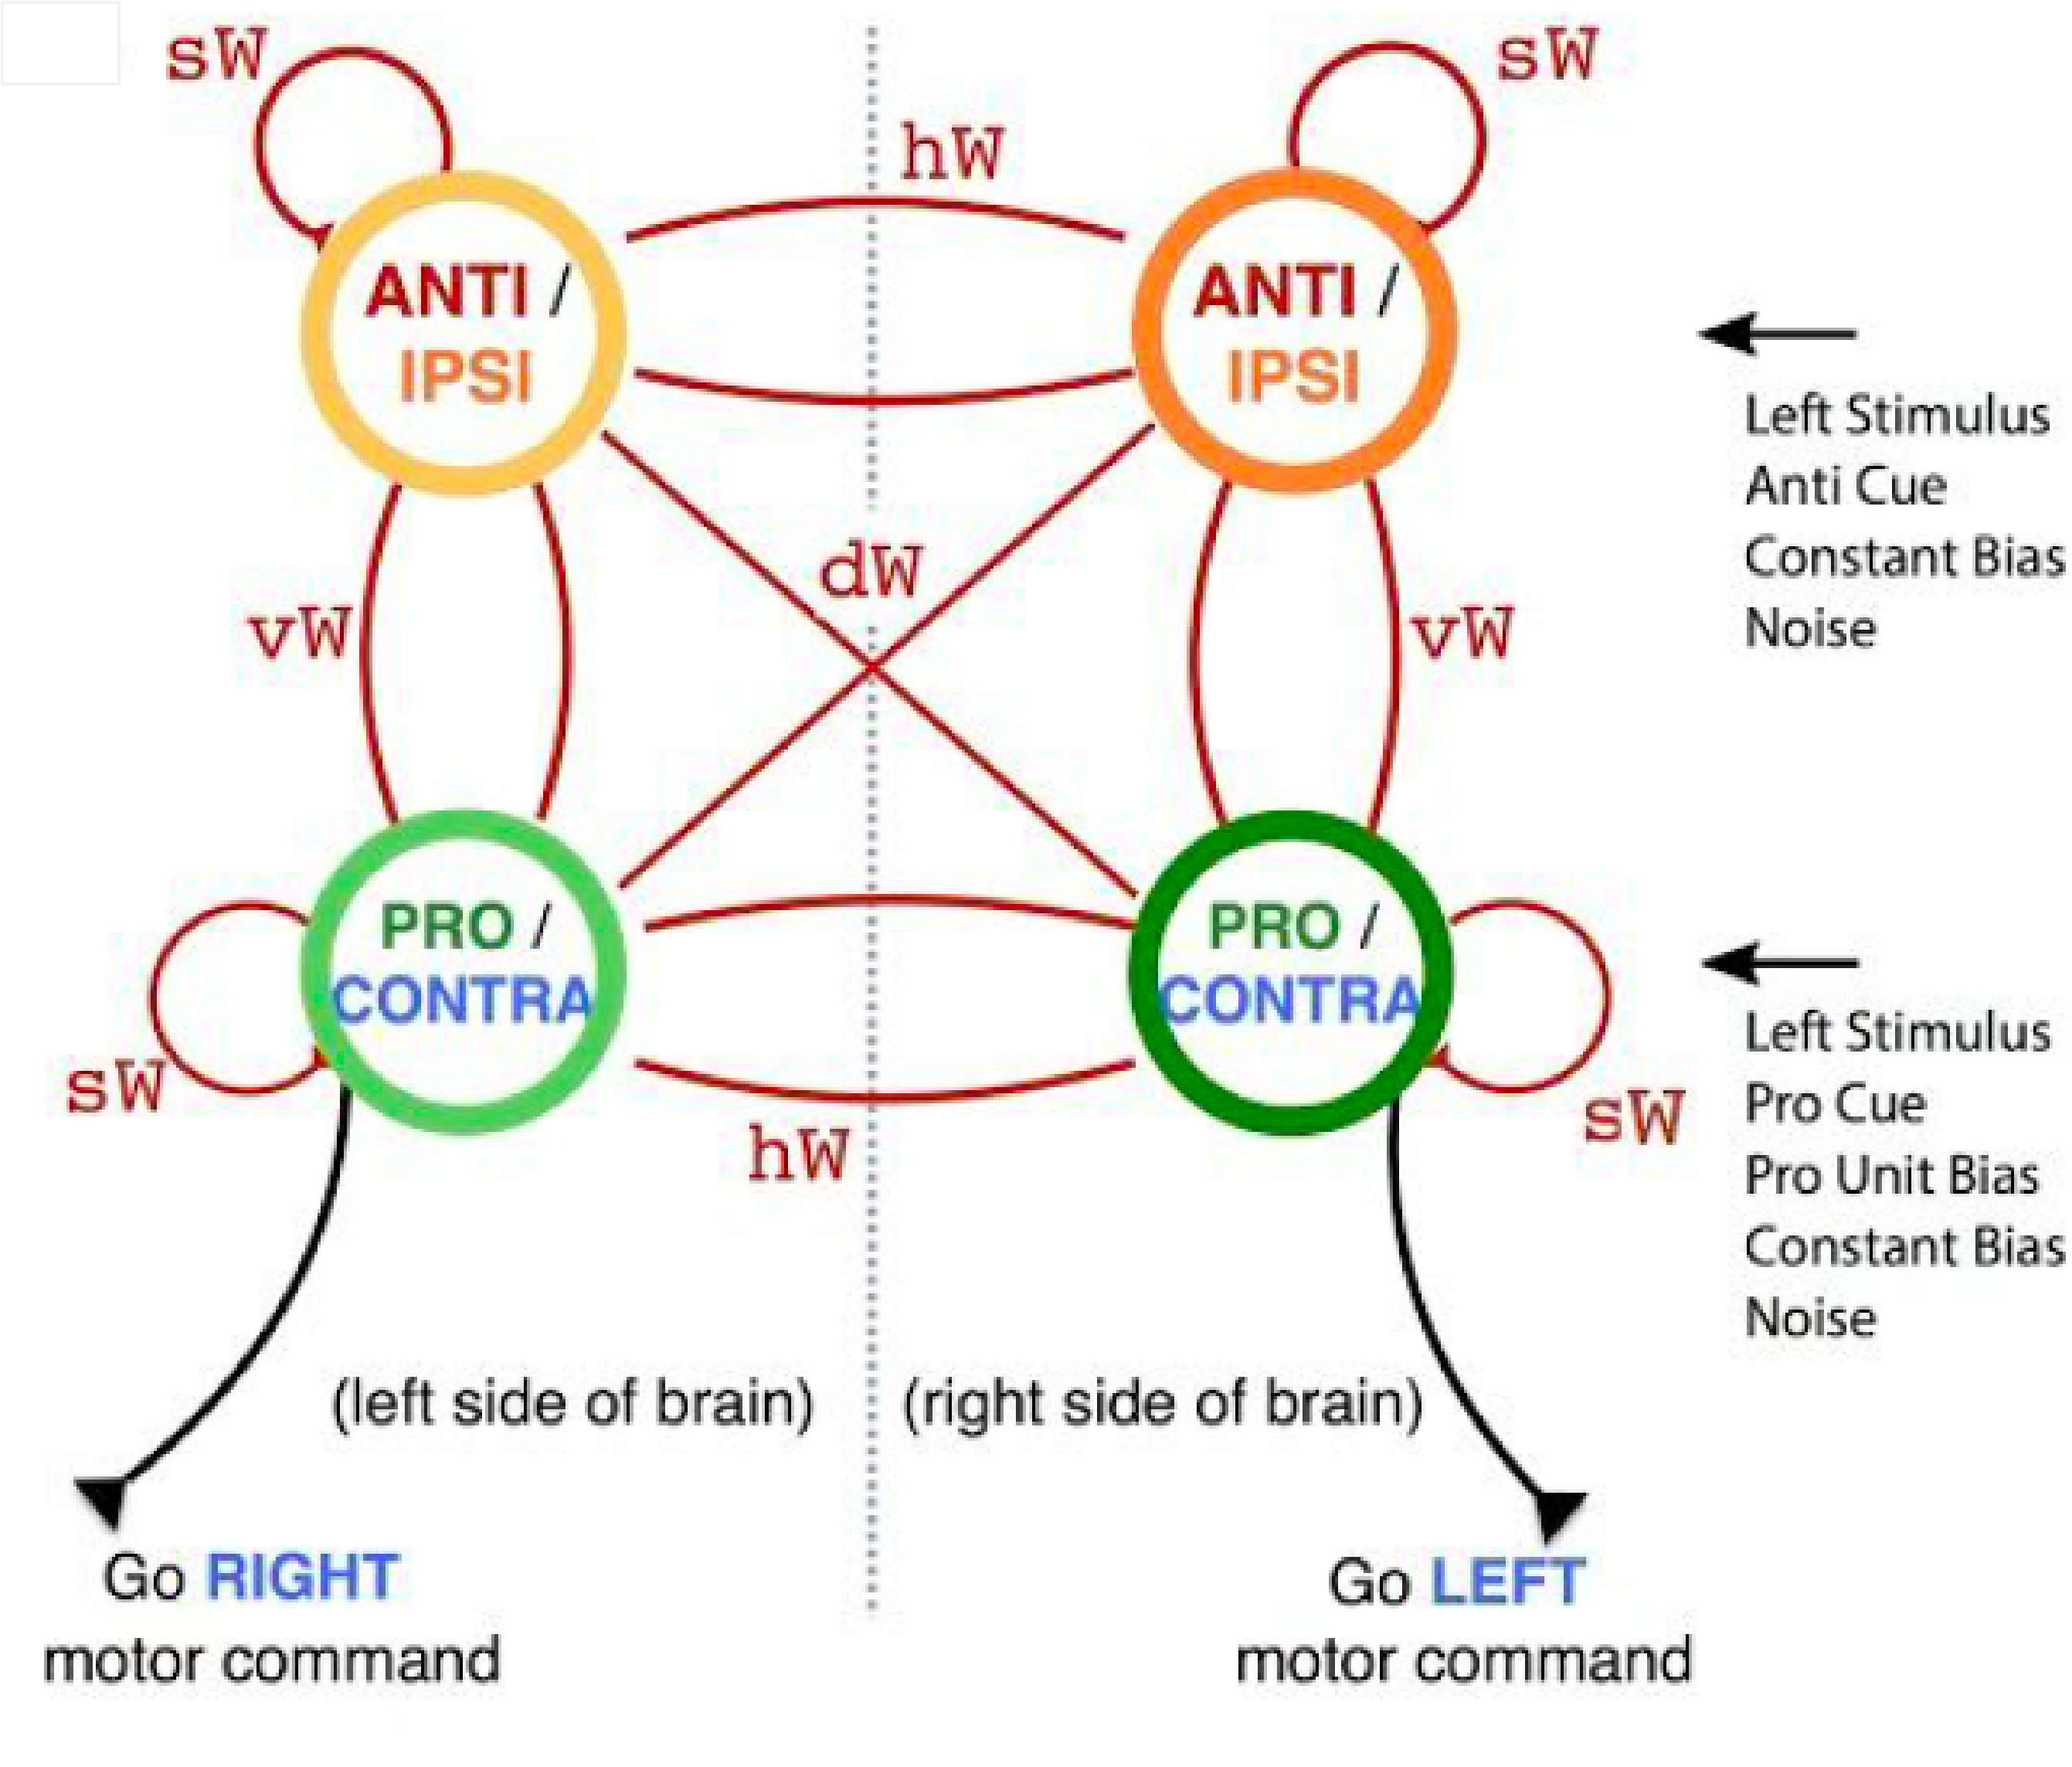
\includegraphics[scale=.3]{figs/Duan_2019_Fig6_clean.png} 
\end{center}
\end{wrapfigure}
The authors designed a nonlinear dynamical model of SC (Fig. 3) and found parameterizations which yielded a high-level description of these experimental results.

There are four total units: two in each hemisphere corresponding to the PRO/CONTRA and ANTI/IPSI populations.  Each unit had an external ($V_i$) and internal ($U_i$) variable related by
\begin{equation}
V_i(t) =\eta(t)\left(\frac{1}{2}\tanh\left(\frac{U_i(t) - \theta}{\beta}\right)+ \frac{1}{2} \right)
\end{equation}
$\theta = 0.05$ and $\beta = 0.5$ control the position and shape of the nonlinearity, repsectively, and $\eta(t)$ is the optogenetic inactivation function.

We can order the elements of $V_i$ and $U_i$ into vectors $v$ and $u$ with elements
\begin{equation}
v = \begin{bmatrix} V_{LP} \\ V_{LA} \\ V_{RA} \\ V_{RP} \end{bmatrix} \hspace{2cm} u = \begin{bmatrix} U_{LP} \\ U_{LA} \\ U_{RA} \\ U_{RP} \end{bmatrix}
\end{equation}

 The internal variables follow dynamics:
\begin{equation}
\tau \frac{\partial u}{\partial t} = -u + Wv + I + \sigma \partial W
\end{equation}
with time constant $\tau = 0.09s$ and gaussian noise $\sigma \partial W$ controlled by the magnitude of $\sigma$.  The weight matrix has 8 parameters $sW_P$, $sW_A$, $vW_{PA}$, $vW_{AP}$, $hW_P$, $hW_A$, $dW_{PA}$, and $dW_{AP}$,  related to the depiction in Fig. 2:
\begin{equation}
W = \begin{bmatrix} sW_P & vW_{PA} &  dW_{PA} & hW_P \\ vW_{AP}  & sW_A & hW_A  & dW_{AP} \\ dW_{AP} & hW_P & sW_A & vW_{AP}  \\  hW_A & dW_{PA} & vW_{PA}  & sW_P \end{bmatrix}
\end{equation}

The input is a sum of five constant scalar parameters:
\begin{equation}
I = I_{\text{constant}} + I_{\text{pro-bias}} + I_{\text{rule}} + I_{\text{choice-period}} + I_{\text{light}}
\end{equation}

\section{Next steps using DSNs}
\textbf{5.1. Free parameters} \\
Our eventual goal is to train a DSN to learn a max-ent distribution on 
\begin{equation}
z = \begin{bmatrix} \theta \\ \beta \\ \sigma \\ sW_P \\ sW_A \\ vW_{PA} \\ vW_{AP} \\ hW_P \\ hW_A \\ dW_P \\ dW_A \\ \tau \\ I_x \\ .. \end{bmatrix}^{\top}
\end{equation}
producing some emergent property.  To do an initial proof of concept, we'll start by fixing many of these parameters to something reasonable, and learning a DSN on say 4-8 variables of interest for tractability of interpretation/validation in the initial stages.  I think it makes sense to start with
\begin{equation}
z = \begin{bmatrix} sW_P \\ sW_A \\ dW_P \\ dW_A \end{bmatrix}
\end{equation}
or
\begin{equation}
z = \begin{bmatrix} sW_P \\ sW_A \\ vW_{PA} \\ vW_{AP} \\ hW_P \\ hW_A \\ dW_P \\ dW_A  \end{bmatrix}
\end{equation}
and fix the rest of the parameters to something reasonable.  Is there a better/more interesting first set of parameters to work with?

\textbf{5.2. Statistically specifying the behavior -- task responses} \\
We are interested in finding model parameterizations, which yield high accuracy in Pro trials across no inacitviation (NI), delay period inactivation (DI), and choice period inactivation (CI).  Additionally, we want high accuracy on Anti trials during NI and CI, but low accuracy during DI.

In the manuscript, this was done by training SC models for many parameterizations, and keeping track of the parameterizations that yielded the task performance just described.  This procedure gives us a set of satisfactory parameterizations, which can be analyzed and examined to gain an understanding of the parameterizations that produce these results and the different possibilities of response types.  

With DSNs, we can use machine learning to find a maximally expansive distribution of such model parameterizations that produce the desired task responses.  This distribution on parameterizations gives us additional insight to the structure of the degenerate space of parameters that produces those task responses.  DSNs  facilitate complementary analyses for understanding the implications of all SC models that produce these responses.

\textbf{5.1 Training a DSN on the SC model and results} \\
Let $V_\alpha,{\text{ss}} = V_\alpha(t = 1.85)$ be the activity of neuron type $\alpha \in \left[LP, LA, RA, RP \right]$ (ss means steady-state), where we have a 1.2 second cue + delay period and a 0.6s choice period.  We want $p_{a,b}$ probability of success ($a \in \left[P, A \right]$ and $b \in \left[NI, DI, CI \right]$), with strong responses -- high or low activity when either succeeding or failing.  In the trained networks of Duan et al. 2019, this either high-or-low response type is encouraged by using term $C_2$ of the cost function (methods of Duan et al. 2019).  With DSNs, we can require that the responses approximately have the properties of Bernoulli variables (which are all or none with some rate).

For a given parameter vector sample $z_i$ from the DSN, let's consider M frozen noise realizations $\sigma \partial W_j \sim \mathcal{N}(0, \sigma) \in \mathcal{R}^T$, where $T = \frac{1.8}{\partial t = 0.024}$.  To encourage the steady state responses of the left and right PRO/CONTRA neurons across the various task conditions to behave as Bernoulli variables, we can ask that for the pro condition with stimulus $s \in \left[L, R\right]$:
\[ E_{\sigma \partial W} \left[ V_{LP,\text{ss}} \mid s=L, b, z_i \right] = \frac{1}{M}\sum_{j=1}^M V_{LP,\text{ss}}(s=L, b, z_i, \sigma \partial W_j) =  p_{P, b} \]
\[ E_{\sigma \partial W} \left[ V_{LP,\text{ss}} \mid s=R, b, z_i \right] = 1 - p_{P, b} \]
\[ E_{\sigma \partial W} \left[ V_{RP,\text{ss}} \mid s=L, b, z_i \right] = 1 - p_{P, b} \]
\[ E_{\sigma \partial W} \left[ V_{RP,\text{ss}} \mid s=R, b, z_i \right] = p_{P, b} \]
$Var_{\sigma \partial W}(V_{LP,\text{ss}} \mid s=L, b, z_i) =   Var_{\sigma \partial W}(V_{LP,\text{ss}} \mid s=R, b, z_i) = Var_{\sigma \partial W}(V_{RP,\text{ss}} \mid s=L, b, z_i) = $ \\
$Var_{\sigma \partial W}(V_{RP,\text{ss}} \mid s=R, b, z_i) = p_{P, b}(1 -  p_{P,b})$

and the analagous equations for the ANTI condition.  As a reminder a Bernoulli random variable $x \in \left[0, 1 \right]$ with parameter $p$ has $E\left[x \right] = p$ and $Var(x) = p(1-p)$.

DSNs enforce statistics in expectation of samples $z_i \sim q_\theta(z_i)$ from the DSN.  So we will end up imposing constraints on the vector:
\begin{equation}
E_{z \sim q_\theta(z)}
\begin{bmatrix}
E_{\sigma \partial W} \left[ V_{LP,\text{ss}} \mid s=L, b, z \right] \\
E_{\sigma \partial W} \left[ V_{LP,\text{ss}} \mid s=R, b, z \right] \\
E_{\sigma \partial W} \left[ V_{RP,\text{ss}} \mid s=L, b, z \right] \\
E_{\sigma \partial W} \left[ V_{RP,\text{ss}} \mid s=R, b, z \right] \\
Var_{\sigma \partial W} \left[ V_{LP,\text{ss}} \mid s=L, b, z \right] \\
Var_{\sigma \partial W} \left[ V_{LP,\text{ss}} \mid s=R, b, z \right] \\
Var_{\sigma \partial W} \left[ V_{RP,\text{ss}} \mid s=L, b, z \right] \\
Var_{\sigma \partial W} \left[ V_{RP,\text{ss}} \mid s=R, b, z \right] \\
... \\
\end{bmatrix}
 = \begin{bmatrix}
p_{P, b} \\
1 - p_{P, b} \\
1 - p_{P, b} \\
p_{P, b} \\
p_{P, b}(1 - p_{P, b}) \\
p_{P, b}(1 - p_{P, b}) \\
p_{P, b}(1 - p_{P, b}) \\
p_{P, b}(1 - p_{P, b}) \\
... \\ 
\end{bmatrix}
\end{equation}

We can additionally control the variance across samples $z$ of these statistics using second moment constraints in addition to the first moment. 

\textbf{5.2 Goal of DSN modeling} \\
Having access to the DSN trained on the SC model and task responses will allow us to make affirmative statements about the model with the desired task performance.  For example, most SC models that produced the appropriate task responses in the manuscript had inhibitory ANTI-PRO connections within hemisphere.  A DSN would allow us to assess frequency of these connections being excitatory or inhibitory in the full parameter space.  Additionally we could examine differences in the remaining parameters/generated activity when those ANTI-PRO within-hemisphere connections are either excitatory or inhibitory. Similarly, one could examine the probability of E vs I connectivity between ANTI and PRO in opposite hemispheres, or the sign of the Schur-decomposition mode contributions. These are some suggestions of many possible analyses that is enabled by having access to the degenerate parameteric distribution.  We should certainly discuss what tests or statements you would like to make moving forward.  Additionally, DSNs (optimized to learn maximum entropy distributions) may identify new parameter regimes for solutions that may be scientifically relevant.


\section{Github}
{\color{blue} \href{https://cunningham-lab.github.io/dsn/}{https://cunningham-lab.github.io/dsn/}} \\

\bibliography{dsn}
\bibliographystyle{unsrt}

\end{document}

